\section*{Übung 3}
\subsection*{Aufgabe 1}
\subsubsection*{Lösungsidee}
Für das tauschen des Inhalts zweier Werte wird eine "`Zwischenspeicher Variable"' benötigt. Der Wert der ersten Variable wird zwischen gespeichert. Danach wird in der ersten Variable der Wert der zweiten Variable gespeichert. Anschließend wird mithilfe der Zwischenspeicher Variable der vorherige gespeicherte Wert von der zweiten Variable übernommen. Das funktioniert bei beiden Datentypen gleich, mit der Ausnahme das die Datentypen in der Prozedur und bei der Übergabe übereinstimmen müssen. 
\newline
\lstinputlisting[language=Pascal] {../swap.pas}
\begin{figure}[H]
	\centering
	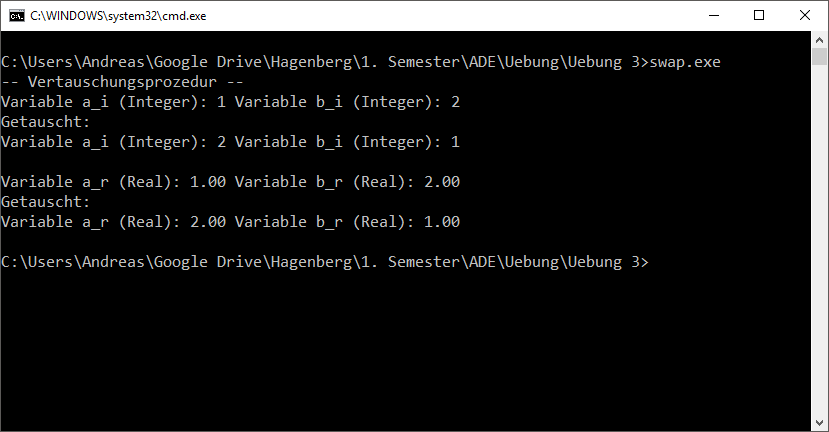
\includegraphics[scale=0.75]{./pictures/swap.png}
	\caption{Testfälle Vertauschungsprozedur}
	\label{fig: Spannweiten Berechnung}
\end{figure}

\section*{Testfälle}
Zum Testen werden vier Variablen mit zwei unterschiedlichen Datentypen initialisiert. Die Variablen mit gleichen Datentyp werden mit unterschiedlichen Werten versehen. Zum Testen werden die Variablen vor - und nach dem tauschen ausgegeben

\newpage

\subsection*{Aufgabe 2}
\subsubsection*{Lösungsidee}
Bei dem Konvertieren einer Dezimalzahl in eine Binärzahl wird folgendermaßen vorgegangen:
\begin{enumerate}
\item Die Zahl durch 2 dividieren
\item Der Rest der Division notieren
\item Falls das Ergebnis nicht 0 ist, Schritt 1 und 2 wiederholen
\item Die umgedrehte Reihenfolge des Restes nacheinander aufgeschrieben ergibt die Binärzahl
\end{enumerate}
Im Programm wird der Rest in $b_{0} .. b_{7}$ gespeichert und anschließend umgekehrt ($b_{7} .. b_{0}$) ausgegeben.
\newline
\lstinputlisting[language=Pascal] {../convert.pas}
\begin{figure}[H]
	\centering
	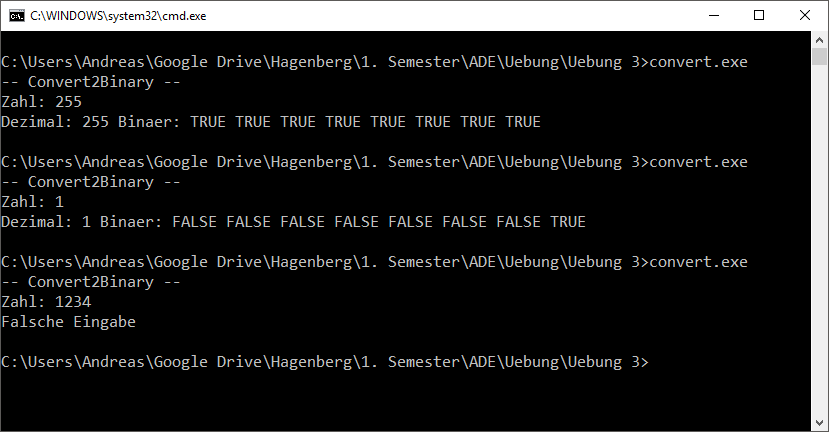
\includegraphics[scale=0.75]{./pictures/convert.png}
	\caption{Testfälle Zahlenkonvertierung}
	\label{fig: Sortieralgorithmus}
\end{figure}

\section*{Testfälle}
Zum Testen werden verschiedene Werte eingegeben, unter anderem auch ein zu hoher Wert.
\newpage

\subsection*{Aufgabe 3}
\subsubsection*{Lösungsidee}
Bei Max2 werden zwei Zahlen miteinander verglichen und das Maximum zurückgegeben. Max3a macht dasselbe mit drei Zahlen und gibt auch das Maximum zurück. Max3b macht sich den Rückgabewert der Max2 Funktion zunutze. Der Funktion werden die ersten beiden Input Zahlen von Max3b übergeben und das Resultat muss nur noch mit der übrigen letzen Input Zahl verglichen werden.
\newline
\lstinputlisting[language=Pascal] {../maxof2or3.pas}
\begin{figure}[H]
	\centering
	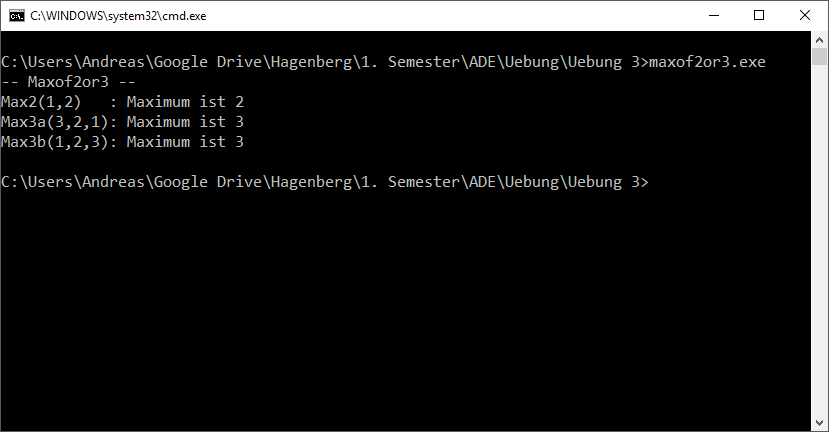
\includegraphics[scale=0.75]{./pictures/maxof2or3.png}
	\caption{Testfälle Maximum von zwei oder drei Zahlen}
	\label{fig: label}
\end{figure}

\section*{Testfälle}
Zum Testen werden Max2, Max3a und Max3b verschiedene Werte übergeben, auch in unterschiedlicher Reihenfolge.
\newpage

\subsection*{Aufgabe 4}
\subsubsection*{Lösungsidee}
Bei dieser Aufgabe muss eine Rundungsfunktion implementiert werden die sich printGraph zunutze macht. Falls das Ergebnis von (num mod 10) größer oder gleich 5 ist wird die zurückgegebene Zahl um eins erhöht. In der printGraph Funktion wird dann für jeweils die Positive und Negative Seite die Anzahl der X ausgegeben. Zusätzlich wird überprüft ob die Summe der Negativen und Positiven Seite nicht 100 überschreitet.
\newline
\lstinputlisting[language=Pascal] {../balkendiagramm.pas}
\begin{figure}[H]
	\centering
	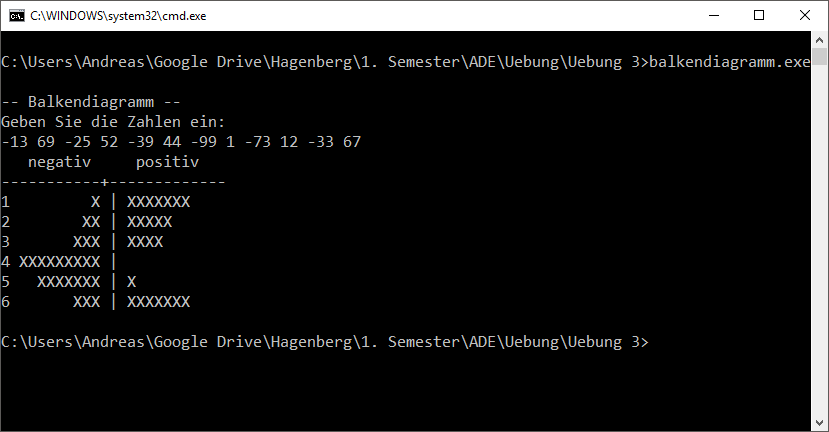
\includegraphics[scale=0.75]{./pictures/balkendiagramm.png}
	\caption{Testfall Balkendiagramm}
	\label{fig: label}
\end{figure}

\section*{Testfälle}
Zum Testen werden verschiedene Werte eingelesen, gerundet und anschließend die Zeilen mit der Anzahl von positiven und negativen X ausgegeben.

\newpage